\documentclass[../resumosTCOM.tex]{subfiles}

\newenvironment{conditions}
  {\par\vspace{\abovedisplayskip}\noindent\begin{tabular}{>{$}l<{$} @{${}={}$} l}}
  {\end{tabular}\par\vspace{\belowdisplayskip}}

\begin{document} 

Uma alternativa equivalente aos NFAs (incluindo $\epsilon$-NFAs) e DFAs.

\paragraph{}

Operações sobre linguagens:
\begin{itemize}
    \item União ($\bigcup$): \(L=\{001, 10\}, M=\{\epsilon, 001\}, LUM=\{\epsilon, 001, 10\}\)
    \item Concatenação (.): \(LM=L.M=\{001, 10, 001001, 10001\}\)
    \item Fecho (*): \(L=\{0, 1\}, L^* é a linguagem das strings binárias\)
\end{itemize}

\paragraph{}

$\epsilon$ e $\emptyset$ são expressões regulares (\(L(\epsilon) = \{\epsilon\}\) e \(L(\emptyset) = \emptyset\))

\paragraph{}

Operadores das Expressões Regulares:
\begin{itemize}
    \item * (zero ou mais)
    \item + (um ou mais)
    \item . (concatenação - pode ser omitido)
    \item Precedência dos operadores: * -> . -> + (podem ser usados parêntesis para forçar uma ordem)
\end{itemize}

\paragraph{}

Todas as linguagens definidas por FAs podem ser definidas por Expressões Regulares e vice-versa:
\begin{figure}[H]
    \centering
    \subfloat{{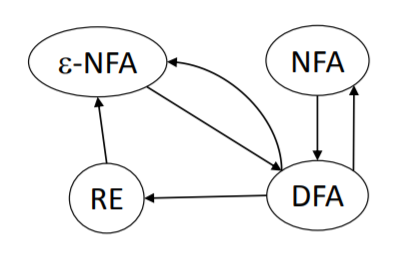
\includegraphics[width=5cm]{images/fa_re.PNG} }}%
    \label{fig:fa_re}%
\end{figure}

\paragraph{}

Dois métodos para converter um DFA numa RE:
\begin{itemize}
    \item Construção de Caminhos (\(R_{ij}^{(k)} = R_{ij}^{(k-1)} + R_{ik}^{(k-1)}(R_{kk}^{(k-1)})R_{kj}^{(k-1)}\))
    \item Eliminação de Estados
\end{itemize}

\paragraph{}

Duas REs são equivalentes se definem a mesma linguagem.

\paragraph{}

Regras/Leis algébricas para REs:
\begin{itemize}
    \item Identidade: \(\emptyset + L = L + \emptyset = L\); \(\epsilon L = L \epsilon = L\)
    \item Absorção: \(L \emptyset = \emptyset L = \emptyset\)
    \item Distributiva: L(M + N) = LM + LN
    \item Idempotência: L + L = L
    \item \((L^*)^* = L^*, \emptyset^* = \epsilon; \epsilon^* = \epsilon; L^+ = LL^* = L^*L; L^* = L^+ + \epsilon\)
\end{itemize}



\end{document}

